\documentclass{article}
\usepackage{graphicx} % Required for inserting images
\usepackage[style=ieee]{biblatex}
\usepackage[letterpaper, total={7in, 9in}]{geometry}
\addbibresource{ref.bib}
\renewcommand*{\bibfont}{\footnotesize}

\begin{document}
\title{Converting Molecular Model Images to Digital Representations}


\author{Wenqi Marshall Guo\\
Department of CMPS\\
University of British Columbia\\
Kelowna, BC\\
wg25r@student.ubc.ca 
\and
Mohamed Shehata\\
Department of CMPS\\
University of British Columbia\\
Kelowna, BC\\
mohamed.sami.shehata@ubc.ca
}

\maketitle


\begin{abstract}
The abstract goes here.
\end{abstract}


\section{Introduction}
Molecular models are helpful tools in chemistry education as they provide an intuitive way for students to understand the 3D structure compared to 2D molecular structure representation. These models can also assist students with 3D mental operations. 
% Although virtual models could be as effective as concrete models, concrete should be available to students at least at the beginning of the study of new concepts and ideas, as humans sometimes rely on concrete objects.\autocite{savec_evaluating_2005} 
A study \cite{savec_evaluating_2005} found that virtual models could has the same effectivness as concrete models, students should have access to concrete models at least at the begining of study because sometimes human rely on concrete objects.  
However, digital model representation has the benefit that allowing students to look up more information about the molecule such as the IUPAC name and the boiling point. Students can also modify the molecule and observe how it will affect the molecular properties. Thus, it will be beneficial if students can convert concrete molecular models to digital representations. 

Although there are models that can convert 2D molecular structure representations to corresponding digital representations \autocite{swinocsr}\autocite{decimer}\autocite{chempix}, to the best of our knowledge, there is not a model for 3D molecular models. It will be beneficial to chemical education to close this gap between 3D molecular models and digital representations. 

Our contribution to this paper can be summarised as:
\begin{itemize}
\item We have constructed two datasets: one computer-rendered 3D molecular model and another consisting of real-world 3D molecular models.
\item We trained a model on top of these two datasets that is capable of converting images of concrete molecular models into their respective SMILES notations. 
\item We applied a method based on multi-image input and beam search to increase the accuracy of the output.
% \item We applied a multi-image input method allowing users to capture multiple images of the molecular model to increase the accuracy of the output.
\end{itemize}

\section{Related Work}
To the best of our knowledge, there is no prior model that can convert a 3D molecular set photo into its digital structure representation. However, there are some models for 2D structure formulas. The two most recent ones are Swin-OCSR\autocite{swinocsr} and DECIMER.ai\footnote{The name DECIMER has been used by the same team for both the dataset and two versions of the mode, here we are refreshing the model published in 2023.}\autocite{decimer}. These two models are very similar in architecture consisting of an image encoder and a transformer.

% The decoder used in 
\subsection{DECIMER.ai}
In DECIMER.ai, the encoder is an EfficientNet-V2-M. EfficientNet is a type of convolutional neural network (CNN) with MBConv \autocite{tan_efficientnet:_2020} (a modified version of the inverted bottleneck from \autocite{mobilenet}) and Fused-MBConv \autocite{suyog_efficientnet-edgetpu:_2019} developed by training-aware neural architecture search (NAS). \autocite{swin_tran} \autocite{effv2} MBConvs have 1x1 point-wise and 3x3 depth-wise convolutional layers, which can yield better parameters and computational efficiency. \autocite{mobilenet} \autocite{effv2} However, they cannot fully utilize modern hardware accelerators. In Efficient-Net-V2, they proposed using regular 3x3 convolutional layers (Fused-MBConvs) to replace MBConvs for the early stages of the network. This results in better training time with small overheads of parameters and FLOPs. In an MBConv block used in Efficient-Net-V2, the image is first passed through a 1x1 convolutional layer to increase its channel numbers, then a squeeze and excitation (SE) block is used \autocite{hu_squeeze-and-excitation_2019}\autocite{tan_efficientnet:_2020}. SE blocks are shown to increase the performance of CNNs with slight computational overhead. \autocite{hu_squeeze-and-excitation_2019}. The SE block is followed by a depthwise 3x3 convolution and a 1x1 convolution, the latter decreases the channel counts to the same as input. In a Fused-MBConv, however, the depthwise convolution and the 1x1 convolution are replaced by a 3x3 convolution. \autocite{effv2} \autocite{mobilenet}

The decoder in DECIMER.ai is a transformer model based on \autocite{attention_is_all_you_need}. It has four transformer encoder blocks and four transformer decoder blocks with right parallel attention heads. \autocite{decimer} The encoder of the transformer utilizes a multi-head self-attention block and an MLP (multilayer perceptron) to replace previous recurrent neural or convolutional layers. The decoder of the Transformer is auto-regressive, meaning the decoder of the model takes in the already generated sequence and predicts the next token. The generated sequence will be processed by a masked multi-head self-attention. The mask will prevent the model from attending tokens after $t$ when generating the $t$-th sequence. Then a cross-attention layer is applied that connects the input sequence and the generated sequence by using the output of the encoder as keys and values and output from the masked self-attention as the query. Then the output of the cross-attention is followed by an MLP layer. The encoder and decoder blocks are repeated for $N$ (In DECIMER.ai $N=4$) times each. After the last decoder block, the output goes through a linear and a softmax layer before output. Since attention does not consider position information, position encoding is added to the sequence for both input and generated sequences. The full transformer also uses residual connection across all the attention and MLP layers. After the addition of the residual connection, a layer normalization is used. A detailed architecture of the Transformer can be found in the original paper \autocite{attention_is_all_you_need}. 

Although DeepSMILES \cite{oboyle_deepsmiles:_2018} has been proposed for machine learning models to generate more valid identifies, their pervous work \cite{rajan_performance_2022} has shown that SMILES actually lead to the most accurate identifiers. Thus, they used SMILES instead of DeepSMILES in DECIMER.ai. \cite{decimer}  
%how it trained on real data and handwritten 
\subsection{Swin-OCSR}
In Swin-OCSR, the encoder (they referred to as "backbone" in their paper) is built on the Swin Transformer. The image is cut into patches with each path having a size of $4 \times 4$ pixels. Then each patch is flattened into and treated as a token which is a 48-dim vector. Then a linear projection layer is applied and each token is into a 192-dim space. 
Then 4 Swin-Transformer (Shifted Window Transformer) \autocite{swin_tran} blocks are used. Each swim transformer block contains two regular transformer modules. In the first transformer module, Window Mutli-head Self Attention (W-MSA) is performed within each window, which is a group of neighbouring tokens. In the second transformer module, the Shifted Window Mutli-head Self Attention (SW-MSA) is performed on a shift-ed window. The W-MSA allows the model to capture the local relationship in the image, and the SW-MSA introduced a cross-window connection while maintaining efficiency. After each block, a patch merging operation is performed such that neighbouring patches are merged and the tokens are contacted. \autocite{swin_tran} \autocite{swinocsr}

% Moved down here To this point, we get a tensor of $\frac{H}{4} \times \frac{W}{4} \times 48$ where $W$ and $H$ are the width and height of the original image. 
% Before the tensor ($H_i \times W_i \times C_i$) gets passed to the next Swin Transformer block, a patch merging operation is performed to capture hierarchical information. During path merging, neighbouring $2 \times 2$ patches are merged and the tokens are concatenated. This results in $\frac{1}{4}$ of the number of patches and each $4C_i$ feature for each token. Then the dimensions of each token are reduced to $2C_i$. In Swin-OCSR, 4 Swin Transformer blocks are used; the last Swin Transformer block outputs a tensor with shape $\frac{H}{32} \times \frac{H}{32} \times 1536$. This tensor is flattened across the spatial axes and projects the last axis into 256 dimensions. 

%how it trained using a special loss function  
% deepsmiles

\section{Method}
\subsection{Synthetic Dataset}
\begin{figure}
    \centering
    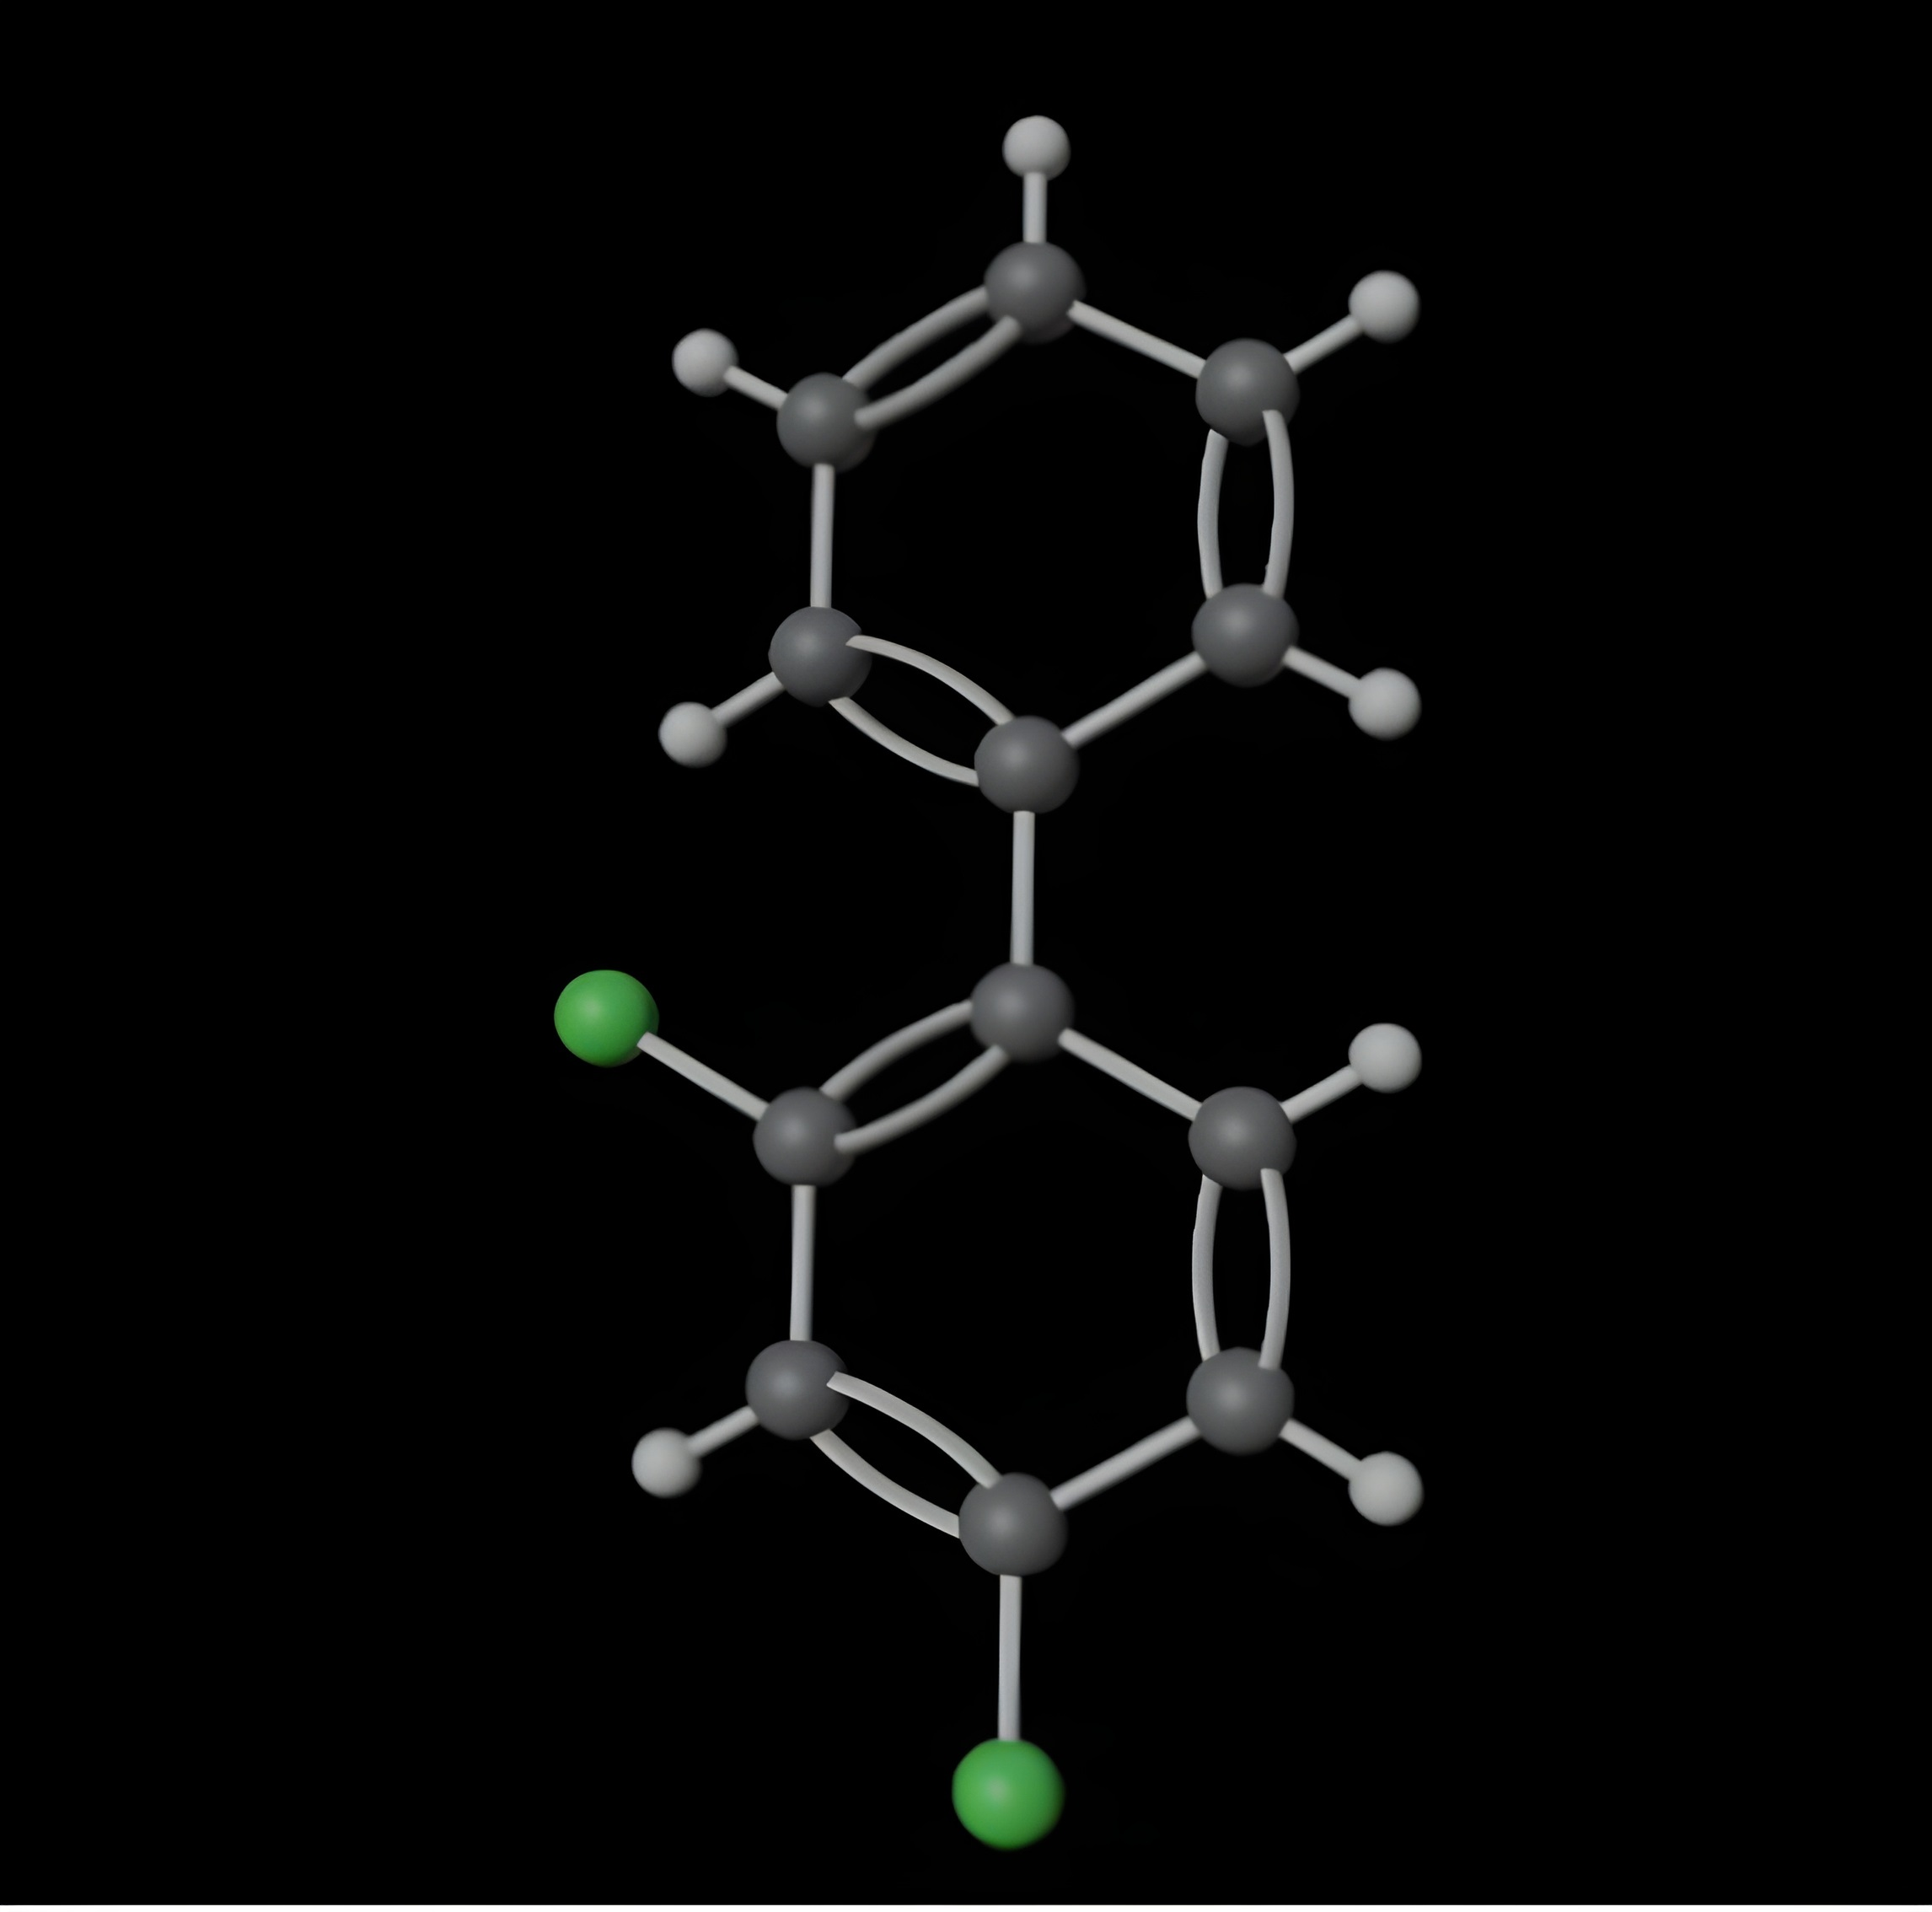
\includegraphics[width=0.3\textwidth]{generated}
    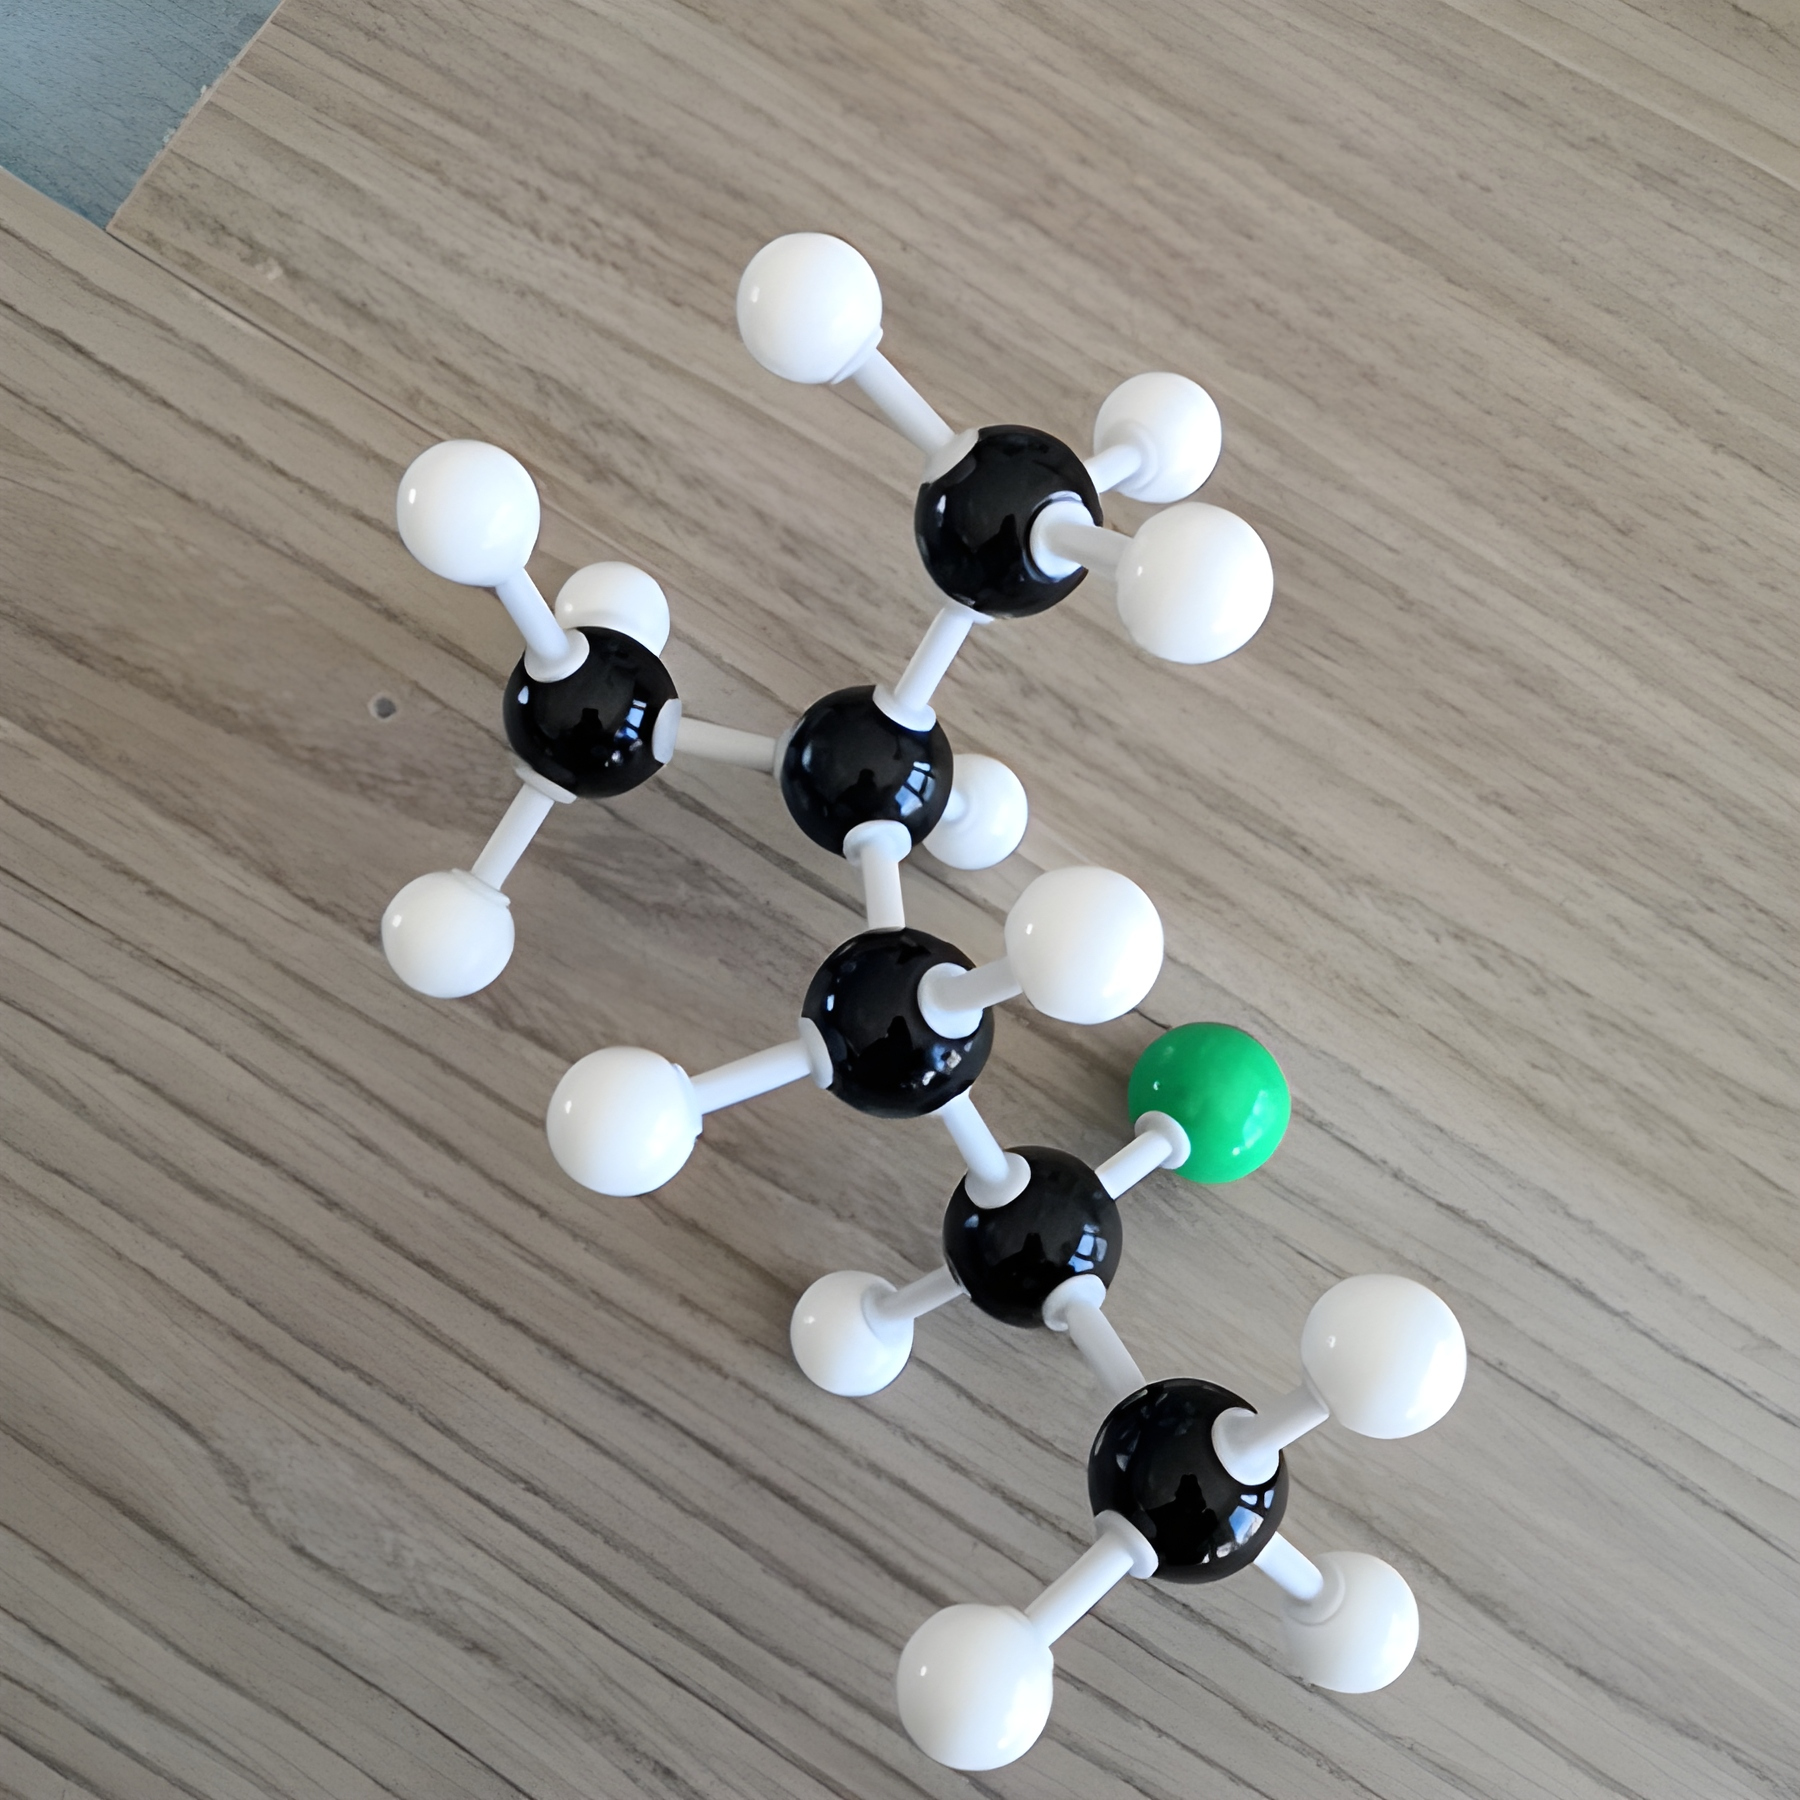
\includegraphics[width=0.3\textwidth]{cap}
    \caption{A rendered image of 2,4-Dichlorobiphenyl and real captured image of 2-Chloro-4-methylpentane}
    \label{fig:example}
\end{figure}

We downloaded a set of compounds from PubChem \autocite{kim_pubchem_2023}, and then these compounds were filtered based on heavy atoms and molecular weights and only contains elements of C, O, S, H, N, Cl, Br, F, and P.
% filtered such that the compounds have at most X atoms \footnote{We did not directly limit the number of atoms on PubChem queries: we limited the number of heavy atoms and molecular weight, which yielded in the limitation of atoms.} 
After filtering, there are 79,369 compounds in the dataset. The pre-train training and validation sets are sperated by images IDs. We created a Blender Python Script to render these compounds into 3D molecular images. OpenAI ChatGPT was used to write the building blocks (API Wrapper) and some logic of the script. The colour of each atom follows the CPK colouring convention and was according to a couple of online sources and 3D molecular models on the market. For each molecule, we rendered 4 different images at different angles. Detailed render process can be found in our GitHub repository. 

%redo
We observed that image size will effect the convergance speed of the model and tradional image size used for classification ($224\times224$) is not enough for our task; thus, we used an image size of $400\times400$. 
\subsection{Real-World Dataset}
We created a mobile application using React.js for data collection. To increase the efficiency of data collection, we group similar models using the GPT: a list of the names of the molecules is given to the GPT via the OpenAI API and asked to group similar molecules together. Users can build either the given molecules or another molecule they chose. Volunteers are recurted to collect these images of molecular models. Because some of the molecular model kit we used dose not have sulfur, we exclude all molecules with sulfur. After collecting, we observed some low quility data such as images with obstruction between atoms, motion blur, etc. Thus, we made another application allowing volunteers to go through all the images and decide if it will be kept or discarded.

We separated the training set and validation set by SMILES strings (i.e. different images of the same molecule will not appear in both validation and traing set. Since we ignored isotopes here, molecules with different IDs might have the same SMILES) The validation set is randomly selected such that it has 20 molecules and 214 images total. 

The images are collected on clear backgrounds, and for each molecule images with different camera angles are captured. In total, we have a total of X images of Y molecules.  

Figure \ref{fig:example} shows an example of rendered and real images. These images are images from dataset after super resolution for better visulation. 
\subsection{Machine Learning Model} 
\begin{figure}
    \centering
    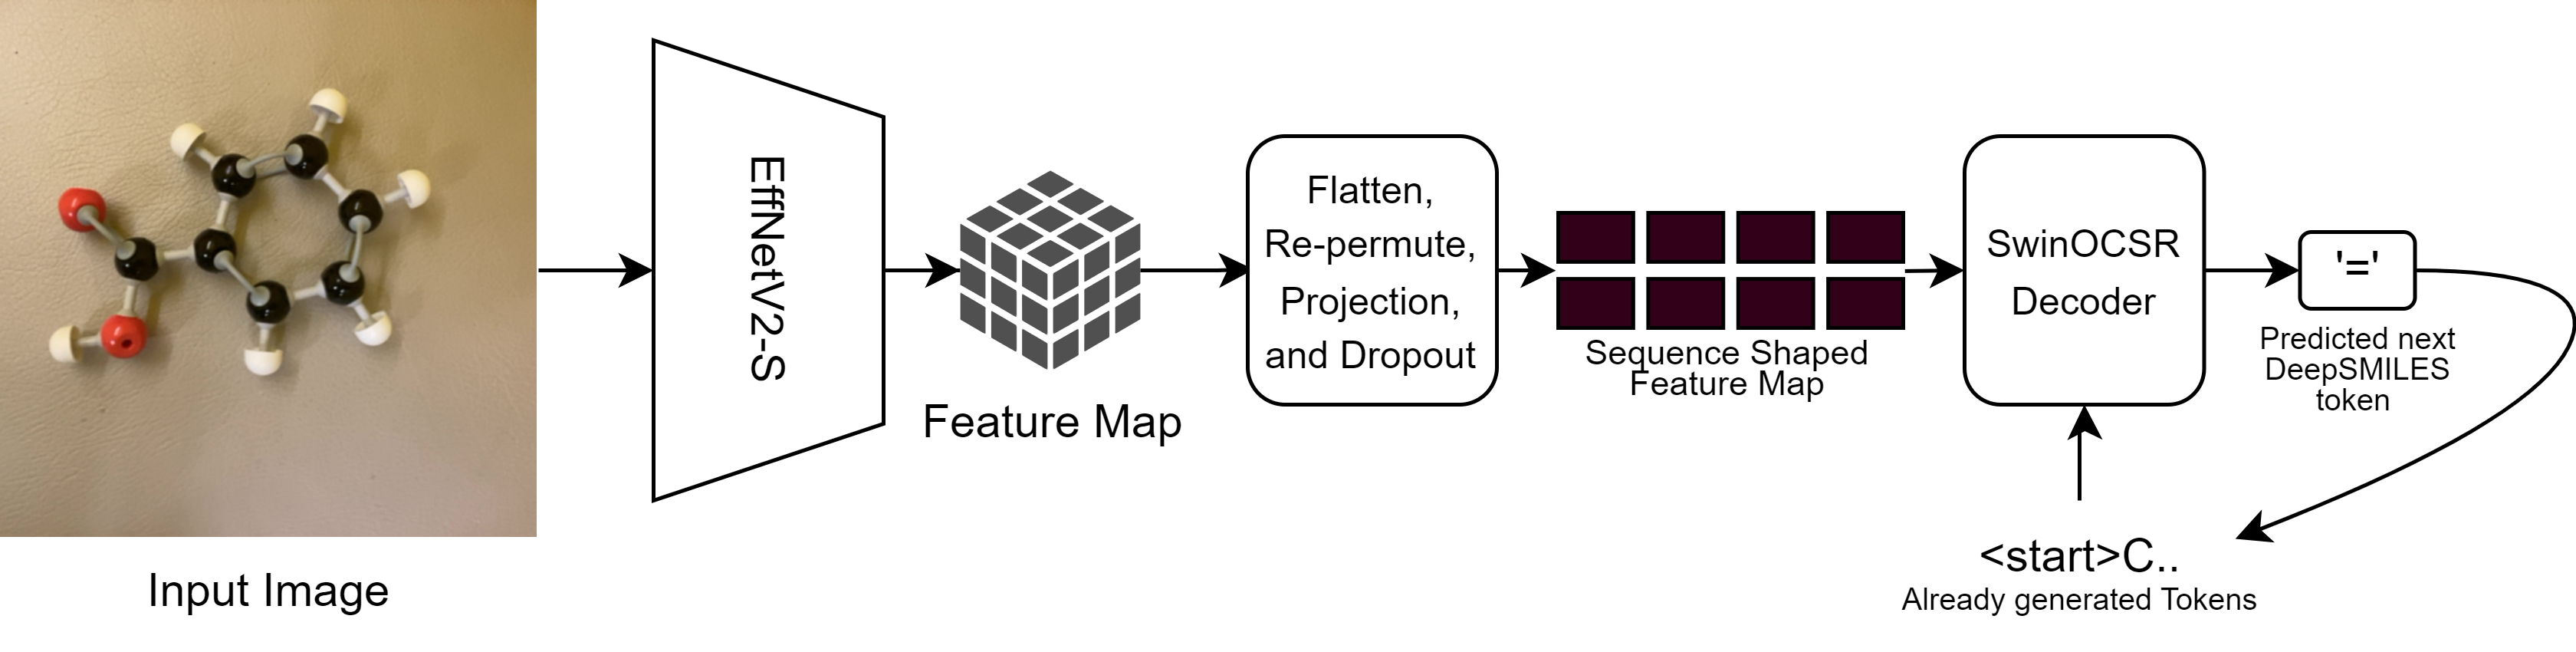
\includegraphics[width=0.9\textwidth]{arch}
    \caption{Model Architecture}
    \label{fig:arch}
\end{figure}
Our model architecture shown in Fig \ref{fig:arch} and  is very similar to the ones used in DECIMER.ai \autocite{decimer} and Swin-OCSR \autocite{swinocsr}. The encoder we used is the EfficientNet-V2-S \autocite{effv2} from torchvision \autocite{torchvision2016} with intinal parameters that trained on ImageNet-1k \autocite{imagenet}. We extracted all the convolution layers from the EffcientNet-V2-S to get a feature map with size $1280\times13\times13$  for each batch. This feature map is then flatten into 2D shape $1280\times169$, re-permuted to sequence-like shape $169\times1280$, projected to 256-dimension to match the input shape of SwinOCSR decoder, and passed through a dropout layer. The tensor is then feeded into our decoder. which is adapted from Swin-OCSR \autocite{swinocsr}. 


We pretrain our model on the synthetic dataset with AdamW \cite{adamw} and exponential learning rate scheduler. Hyperparameters are adjusted manuually and the training is stoped when token-level accuracy converges. 

We then fine tune our model on the real-world dataset. With the fixed validation set, we did a hyperparamater sweep using Weight and Bias \autocite{wandb} to select models with highest validation token-level accuracy. Then the hyper-parameter is furture finetuned manually. 

\subsection{Beam search and Mutli-image input}
Beam search is a way to increase the accuracy of autoregressive models. \cite{yang_breaking_2018} \cite{zhang_beam_2024} 
We also hyprothesis that multiple images input will increase the accuracy of the model, shich has shown in pervious research \cite{sun_multi-input_2017}. In \cite{sun_multi-input_2017}, the authors use ``early fusion" method where feature maps from 3 different images are concatenated on channel axis in the early stage of network. However, this method requires modification of the backbone network and the number of images in this method are fixed. Instead, our method passes individual images through the entire network (including the EfficientNet-V2-S and SwinOCSR decoder) and average the softmax distribution of tokens.  
\section{Results}
We tested how the perfomance of our model behevious with different beam size and number of images on a subset of validation set with only molecules that has at least 5 images. 
\begin{figure}
    \centering
    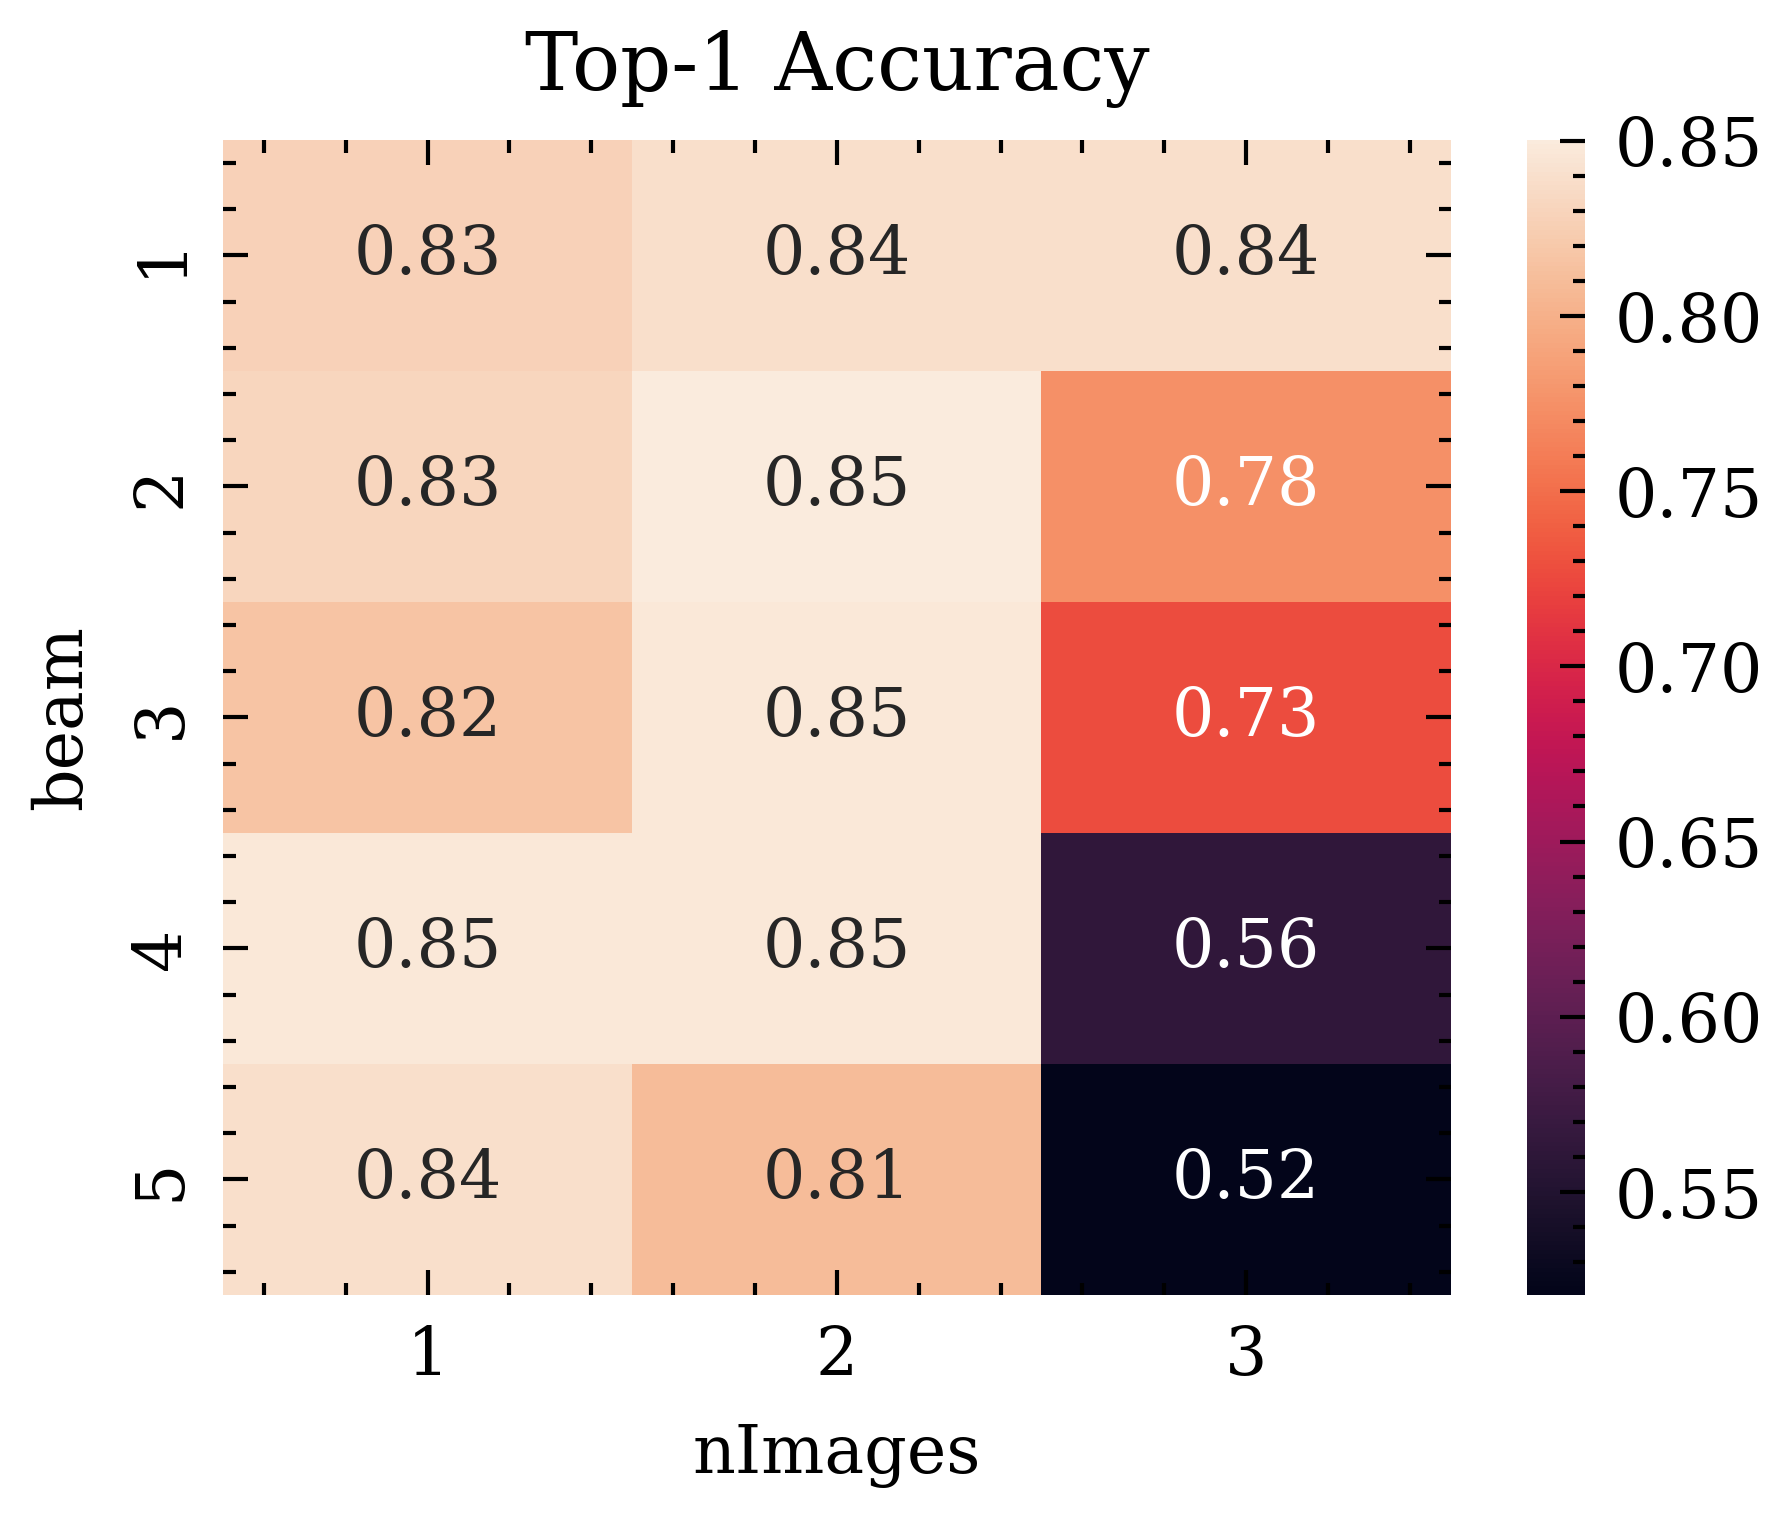
\includegraphics[width=0.3\textwidth]{top1.png}
    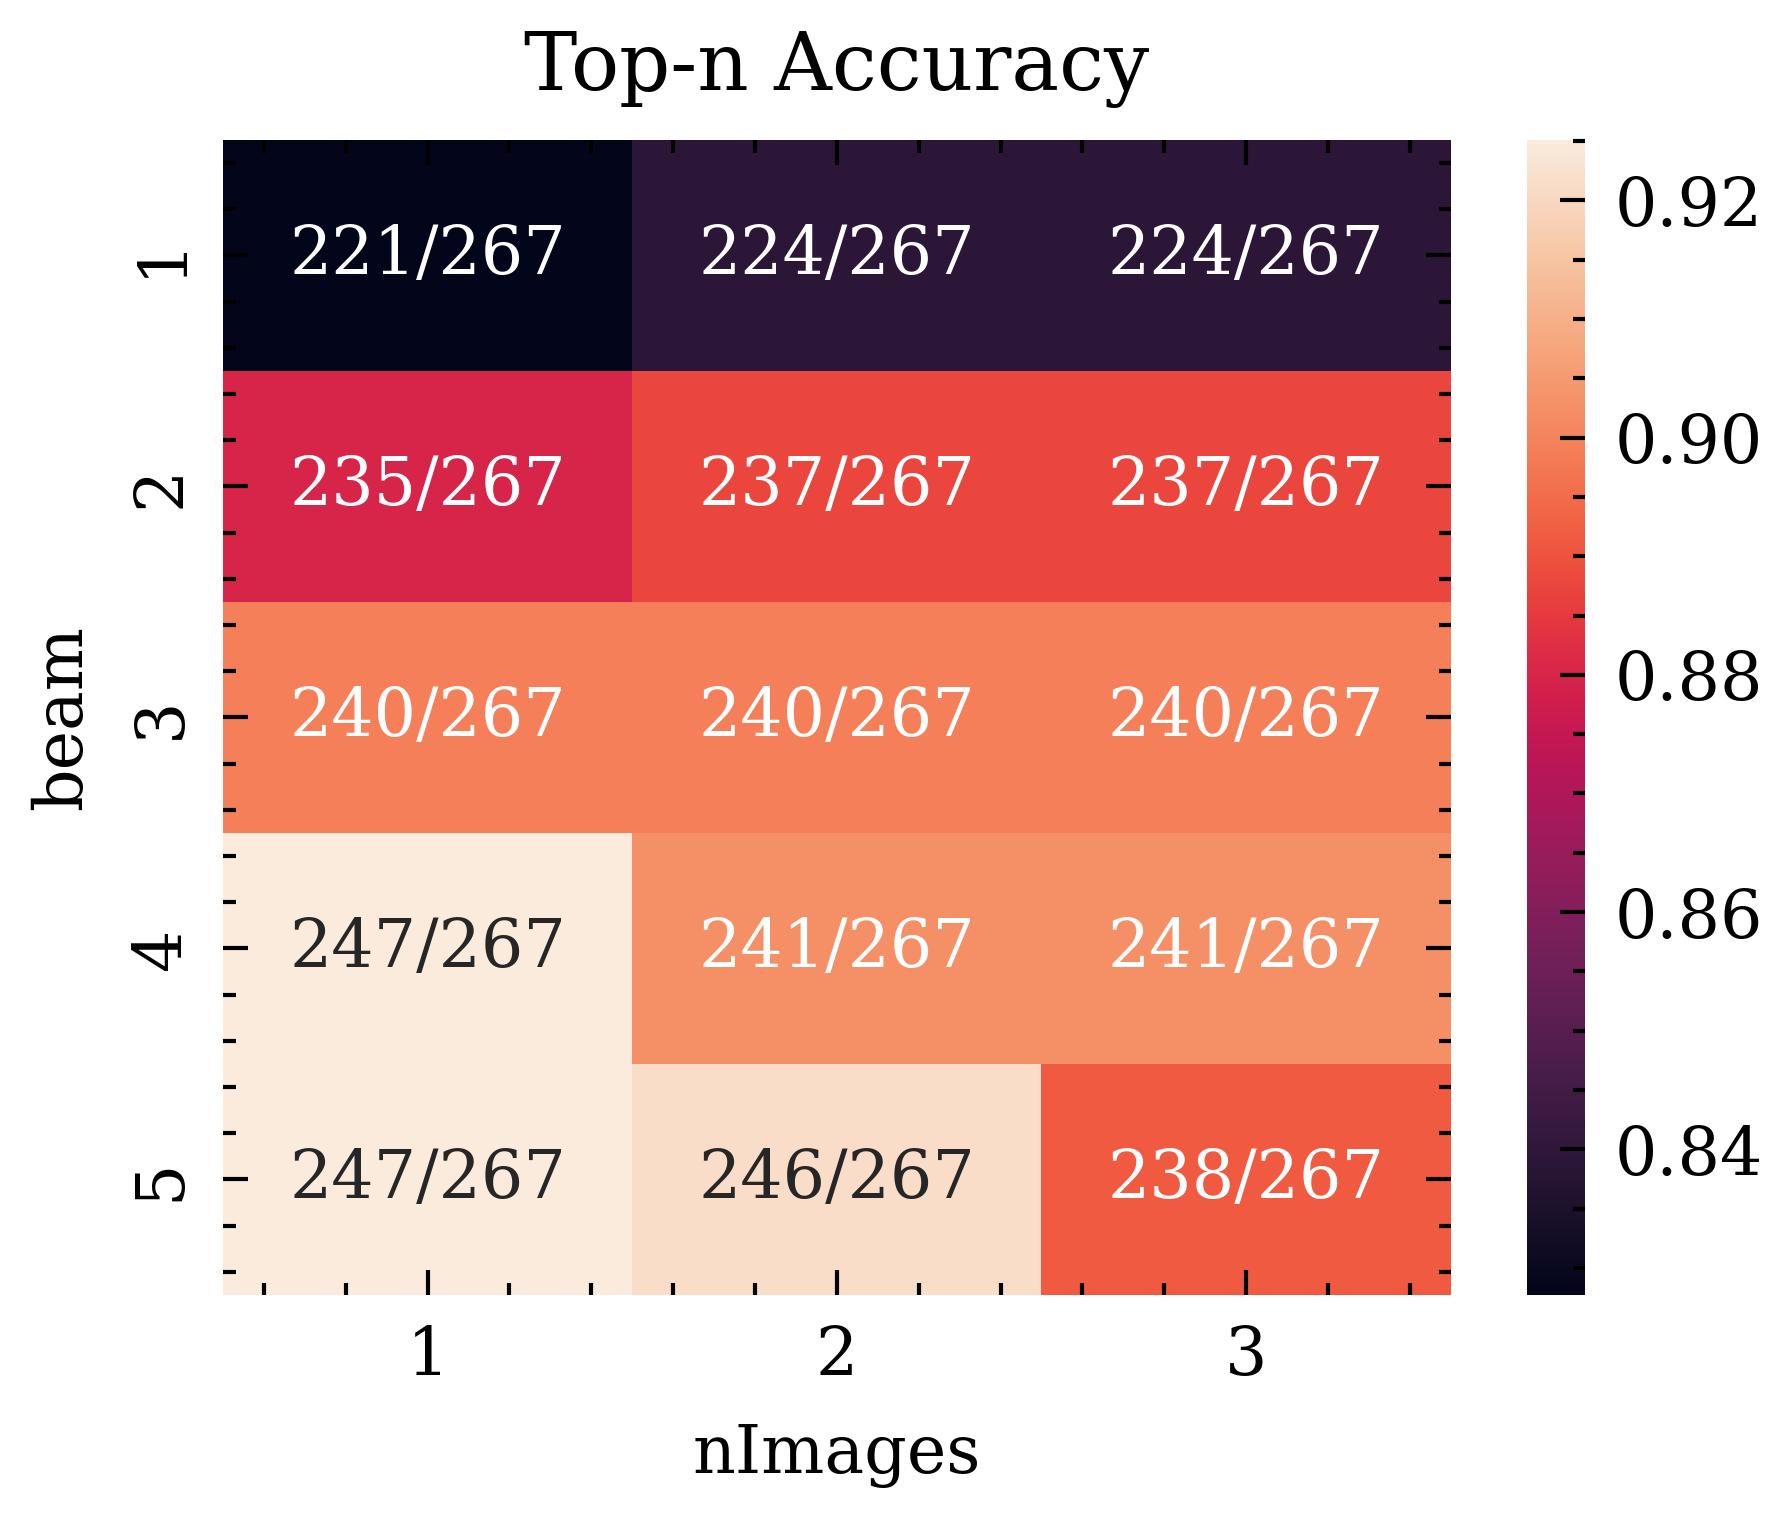
\includegraphics[width=0.3\textwidth]{topn.png}
    \caption{Top 1 and Top-\textit{beam} Sequence Level Accuray (accuracy$\pm$95\%CI)}
    \label{fig:res}
\end{figure}


compare the accuracy of different types of molecules
compare with hand written OCSR 
\section{Conclusion}
\section{Demo}
We deployed the model on our server \footnote{\url{http://file.weasoft.com:8888}} with a frontend and open source our model on github\footnote{\url{https://github.com/weathon/3d2smile}}. 
\section{Limation and Future Work}
In this project, we did not attempt to recognize stereochemical information such as chirality and E/Z structure. However, these are important concepts for students to understand and being able to show these is one of the key characteristics and benefits of 3D models. 
% Additionally, we used multi-image input to increase the accuracy of the model by doing answer voting on the generated sequence. However, ensembling the probability distribution for each token might be a more advanced and better approach, further experiments are needed to select the best approach.
Our real-world dataset is limited by time and budget, a larger dataset could increase the accuracy and robustness of the model. 
%It could also make 3D stereochemical information more recognizable. gpt?
This project only focused on the technical side of the problem and did not test how well this application would be in classroom settings, further chemical education studies are needed to determine its effectiveness in education. 
Traditional molecular models have some limitations, such as they might be misleading and let students think energy is needed to create bonds\autocite{snatoms}. Train a machine learning model on alternative molecular models, such as Snatoms\autocite{snatoms}, might be able to provide better education values.
\section*{Acknowledgement}
The author wants to thank Dr. Brian Ganley from the Chemistry Department of the University of Missouri-Columbia for providing use cases and other advice on this project; Dr. Hung-yi Lee from National Taiwan University and Dr. Mu Li and Dr. Yi Zhu from Amazon for their illuminating lectures on YouTube played an essential role in the process of this project; Peizhi Yan and Dr. Shan Du from the University of British Columbia for mentoring in the process; and Beiliang Zhao from UBC for peer discussion.

The creation of this project was aided by OpenAI ChatGPT and Google Gemini, which contributed to tasks including but not limited to brainstorming, troubleshooting, writing feedback, and coding support.

The computation of this work is mainly performed on UBC Advanced Research Computing, DOI: 10.14288/SOCKEYE.

% \IEEEpeerreviewmaketitle
\printbibliography
\end{document}


